
\documentclass{article}
\usepackage{graphicx}
\usepackage{float}
\begin{document}

%the distribution of data
\begin{figure}[htb]
  % Requires \usepackage{graphicx}
  \centering
  \includegraphics[scale=.8
  ]{BMS-POS.eps}\\
  \caption{BMS-POS}\label{fig:graph}
\end{figure}

\begin{figure}[htb]
  % Requires \usepackage{graphicx}
   \centering
  \includegraphics[scale=.8]{BMS-WEBVIEW.eps}\\
  \caption{BMS-Webview}\label{fig:graph}
\end{figure}

\begin{figure}[htb]
  % Requires \usepackage{graphicx}
   \centering
  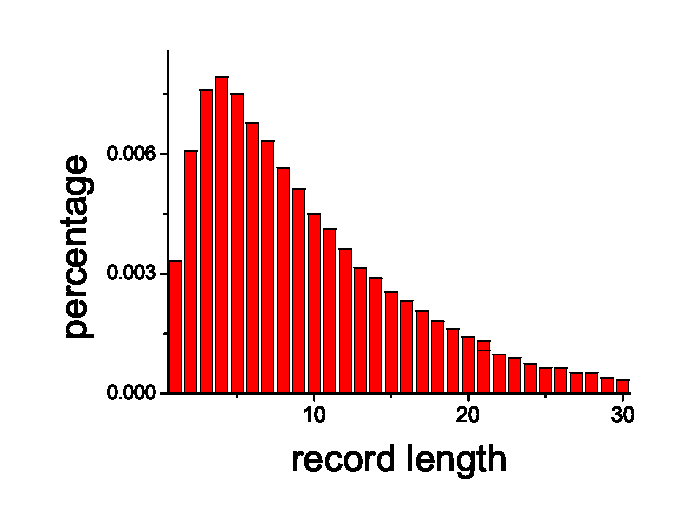
\includegraphics[scale=.8]{retail.eps}\\
  \caption{retail}\label{fig:graph}
\end{figure}

\begin{figure}[htb]
  % Requires \usepackage{graphicx}
   \centering
  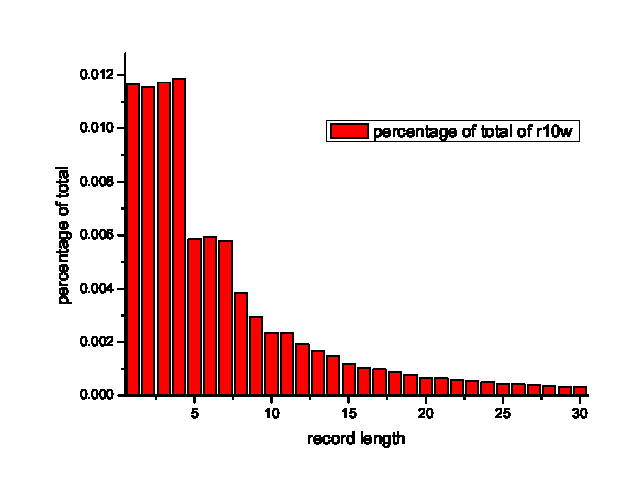
\includegraphics[scale=.8]{r10w.eps}\\
  \caption{r10w}\label{fig:graph}
\end{figure}

\begin{figure}[htb]
  % Requires \usepackage{graphicx}
   \centering
  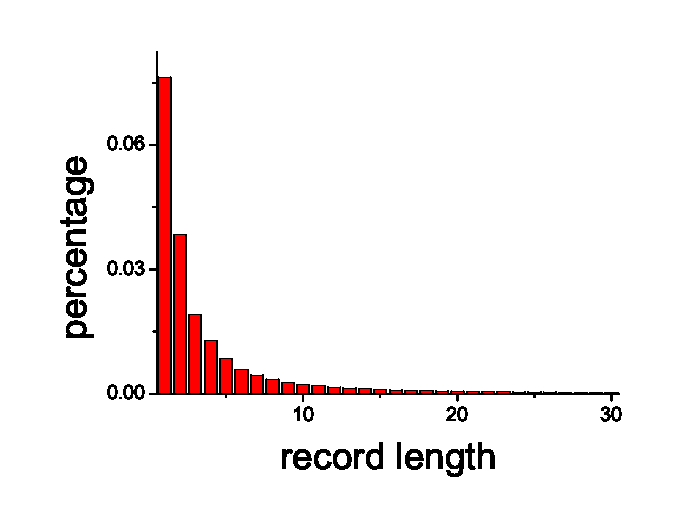
\includegraphics[scale=.8]{r50w.eps}\\
  \caption{r50w}\label{fig:graph
  }
\end{figure}
As we can see from the graph, the characteristic of the distribution of all data sets is that the longer the record is, the less they account for.Although there are some anomalies in retail since it's quite impossible for people to buy only one thing in a supermarket, the distribution remains the same after the record length comes to four. The following graphs show the distribution of nonsensitive items.














%the distribution of  nonsensitive item
\begin{figure}[htb]
  % Requires \usepackage{graphicx}
  \centering
  \includegraphics[scale=.8
  ]{bmsnon.eps}\\
  \caption{BMS-POS}\label{fig:graph}
\end{figure}

\begin{figure}[htb]
  % Requires \usepackage{graphicx}
   \centering
  \includegraphics[scale=.8]{wbnon.eps}\\
  \caption{BMS-Webview}\label{fig:graph}
\end{figure}

\begin{figure}[htb]
  % Requires \usepackage{graphicx}
   \centering
  \includegraphics[scale=.8]{retailnon.eps}\\
  \caption{retail}\label{fi
  g:graph}
\end{figure}

\begin{figure}[htb]
  % Requires \usepackage{graphicx}
   \centering
  \includegraphics[scale=.8]{r10wnon.eps}\\
  \caption{r10w}\label{fig:graph}
\end{figure}

\begin{figure}[htb]
  % Requires \usepackage{graphicx}
   \centering
  \includegraphics[scale=.8]{r50wnon.eps}\\
  \caption{r50w}\label{fig:graph}
\end{figure}
The above figures show that the number of nonsensitive items in a record also diminishes dramatically with the length increasing. An exception appears at length 0, which indicates that records composed of only sensitive items still account for a large percentage.









Relative entropy is a value to judge whether two data set is similar with each other. However,there exists a disadvantage in it when the domain of two data sets is different.As a result, we apply symmetric relative entropy to our result.The comparison is as followings.

%table for rho=0.3 total
\begin{table}[htb]
\begin{tabular}{|c|c|c|}
  \hline
  % after \\: \hline or \cline{col1-col2} \cline{col3-col4} ...
    \multicolumn{3}{|c|}{rho=0.3}\\
  \hline
   & TDcontrol & partial \\\hline
  BMS-POS & 0.82204 & 0.05129 \\\hline
  BMS-Webview & 0.16866 & 0.04199 \\\hline
  retail & 0.74499 & 0.11816 \\
  \hline
\end{tabular}
\caption{ relative entropy in original data where rho=0.3}
\end{table}

%table for rho=0.5 total
\begin{table}
\begin{tabular}{|c|c|c|}
  \hline
  % after \\: \hline or \cline{col1-col2} \cline{col3-col4} ...
    \multicolumn{3}{|c|}{rho=0.5}\\\hline
   & TDcontrol & partial \\\hline
  BMS-POS & 0.80801 & 0.0436 \\\hline
  BMS-Webview &0.16598 & 0.03474 \\\hline
  retail & 0.11195& 0.11195 \\
  \hline
\end{tabular}
\caption{ relative entropy in original data where rho=0.5}
\end{table}



%table for rho=0.7 total
\begin{table}
\begin{tabular}{|c|c|c|}
  \hline
  % after \\: \hline or \cline{col1-col2} \cline{col3-col4} ...
    \multicolumn{3}{|c|}{rho=0.7}\\
  \hline
   & TDcontrol & partial \\\hline
  BMS-POS &0.69708 & 0.0435 \\\hline
  BMS-Webview     &0.7636 & 0.03438 \\\hline
  retail    & 0.74499& 0.1119 \\
  \hline
\end{tabular}
\caption{ relative entropy in original data where rho=0.7}
\end{table}


%table for rho=0.3 CutMid
\begin{table}
\begin{tabular}{|c|c|c|c|c|}
  \hline
  % after \\: \hline or \cline{col1-col2} \cline{col3-col4} ...
    \multicolumn{3}{|c|}{rho=0.3}\\
  \hline
   & TDcontrol & partial \\\hline
  BMS-POS-cut50 &0.20164 & 0.05868 \\\hline
  BMS-Webview-cut50 & 0.76934 & 0.04486 \\\hline
  retail-cut50& 0.79641 & 0.11476 \\\hline
  r10w-cut50 &0.78064 & 0.10889\\\hline
  r50w-cut50 & 0.74762& 0.04956 \\
  \hline
\end{tabular}
\caption{ relative entropy in CutMid where rho=0.3}
\end{table}

%table for rho=0.5 CutMid
\begin{table}
\begin{tabular}{|c|c|c|c|c|}
  \hline
  % after \\: \hline or \cline{col1-col2} \cline{col3-col4} ...
    \multicolumn{3}{|c|}{rho=0.5}\\
  \hline
   & TDcontrol & partial \\\hline
  BMS-POS-cut50 &0.20164 &0.0485 \\\hline
  BMS-Webview-cut50 & 0.77182 & 0.03687 \\\hline
  retail-cut50& 0.77546 & 0.10934 \\\hline
  r10w-cut50 &0.1715 & 0.10487\\\hline
  r50w-cut50 & 0.74778& 0.04515 \\
  \hline
\end{tabular}
\caption{ relative entropy in CutMid where rho=0.5}
\end{table}


%table for rho=0.7 CutMid
\begin{table}
\begin{tabular}{|c|c|c|c|c|}
  \hline
  % after \\: \hline or \cline{col1-col2} \cline{col3-col4} ...
    \multicolumn{3}{|c|}{rho=0.7}\\
  \hline
   & TDcontrol & partial \\\hline
  BMS-POS-cut50 &0.76961 &0.04827 \\\hline
  BMS-Webview-cut50 & 0.77548 &0.03659 \\\hline
  retail-cut50& 1.21138 &0.10922 \\\hline
  r10w-cut50 &  N/A &0.10487\\\hline
  r50w-cut50 & 0.75072&0.04519 \\
  \hline
\end{tabular}
\caption{ relative entropy in CutMid where rho=0.7}
\end{table}



Global suppression is unavailable in large data sets. We tested all of the data sets and found that only a small portion can be terminated in 2 hours or can be executed rightly in a limited memory.As a result, we didn't show the result of global suppression in original data sets and CutMid data sets and we only make comparison in small data sets which derived from those original ones with columns length less than or equal to five.



%table for rho=0.3 CutSmall
\begin{table}
\begin{tabular}{|c|c|c|c|}
  \hline
  % after \\: \hline or \cline{col1-col2} \cline{col3-col4} ...
   \multicolumn{4}{|c|}{rho=0.3}\\
  \hline
  &TDcontrol & global & partial \\\hline
  BMS-POS-cut5 & 0.68446&0.22441&0.00307 \\\hline
  BMS-Webview-cut5 &0.38858 &0.65379 &0.32098\\\hline
   retail-cut5 & 0.60346 & 0.32978 & 0.03721 \\\hline
  r10w-cut5 & 0.68009 & 0.17224 & 0.03264 \\\hline
  r50w-cut5 & 0.6097 & 0.17069 & 0.07998 \\\hline
\end{tabular}
\caption{ relative entropy in CutSmall where rho=0.3}
\end{table}





%table for rho=0.5 CutSmall
\begin{table}
\begin{tabular}{|c|c|c|c|}
  \hline
  % after \\: \hline or \cline{col1-col2} \cline{col3-col4} ...
   \multicolumn{4}{|c|}{rho=0.5}\\
  \hline
  &TDcontrol & global & partial \\\hline
  BMS-POS-cut5 & 0.64811&0.28808& 0.0017 \\\hline
  BMS-Webview-cut5 &0.3856&0.63761 &0.31798\\\hline
   retail-cut5 &0.59911 & 0.30997&0.02766 \\\hline
  r10w-cut5 &0.67783& 0.17223& 0.03287 \\\hline
  r50w-cut5 & 0.60964 & 0.17069 & 0.00767 \\\hline
\end{tabular}
 \caption{ relative entropy in CutSmall where rho=0.5}
\end{table}

%table for rho=0.7 CutSmall
\begin{table}
\begin{tabular}{|c|c|c|c|}
  \hline
  % after \\: \hline or \cline{col1-col2} \cline{col3-col4} ...
   \multicolumn{4}{|c|}{rho=0.7}\\
  \hline
  &TDcontrol & global & partial \\\hline
  BMS-POS-cut5 & 0.68846& 0.29457 & 0.00165 \\\hline
  BMS-Webview-cut5 &0.69705 &0.63483 &0.31794\\\hline
   retail-cut5 &0.58437 &0.28068&0.02754 \\\hline
  r10w-cut5 &0.60025& 0.17238& 0.03287 \\\hline
  r50w-cut5 & 0.69361 & 0.17069 & 0.00767 \\\hline
\end{tabular}
  \caption{ relative entropy in CutSmall where rho=0.7}
\end{table}




%table for rules (sup=5 rho=0.7)
\begin{table}
\begin{tabular}{|c|c|c|c|c|}
  \hline
  % after \\: \hline or \cline{col1-col2} \cline{col3-col4} ...
  & original & TDcontrol & global & partial \\\hline
  BMS-POS-cut5 & 4457 &36 & 5& 4007 \\\hline
  BMS-Webview-cut5 & 600& 58  &98 & 249 \\\hline
  retail-cut5 & 674 & 0& 87& 402 \\\hline
\end{tabular}
  \caption{ rules where sup=5 rho=0.7}
\end{table}


%table for rules(sup=10 rho=0.7)
\begin{table}
\begin{tabular}{|c|c|c|c|c|}
  \hline
  % after \\: \hline or \cline{col1-col2} \cline{col3-col4} ...
   & original &TDcontrol & global & partial \\ \hline
  BMS-POS-cut5 & 1814 &24  & 0& 1664 \\ \hline
  BMS-Webview-cut5 & 197&24  &36 & 97 \\ \hline
  retail-cut5 & 217 & 0& 47& 155\\
  \hline
\end{tabular}
\caption{ rules where sup=10 rho=0.7}
\end{table}


%table for rules(sup=20 rho=0.7)
\begin{table}
\begin{tabular}{|c|c|c|c|c|}
  \hline
  % after \\: \hline or \cline{col1-col2} \cline{col3-col4} ...
   & original &TDcontrol & global & partial \\ \hline
  BMS-POS-cut5 & 752 &18  & 0& 702 \\ \hline
  BMS-Webview-cut5 &  68& 4&6 & 28 \\ \hline
  retail-cut5 & 101 &0 & 30& 77 \\
  \hline
\end{tabular}
  \caption{ rules where sup=20 rho=0.7}
\end{table}
Since r10w and r50w are two data sets generated randomly, rules cannot be mined when the support is set at five or even larger.So we just put the real data to make comparison.One point that has to be paid attention is that rules mined by TDcontrol may be totally different from the original ones.For example, if there exists a rule: a b c->1 where a,b and c are generalized items which do not exist in the original domain, such rules cannot be gained in any combination of the original domain. In order to make comparison between partial suppression and TDcontrol in the number of rules, the rules mined by generalization should be transferred into their original forms. Since several items are generalized into one, expanding such an item into its children is reasonable.As the former sample, if a represents {2,3},b represents {4,5} c represents {6}, the rule a b c->1 should be expanded to
2,4,6->1
2,5,6->1
3,4,6->1
3,5,6->1
According to this strategy, a further comparison can be made.
%table



The most widely criticized disadvantage of partial suppression is that it is entirely possible that new rules may appear in the processed data set. Technologically, the generalization method will cause the same problem. We will show the additional rules mined by partial suppression and generalization.

%table for additional rules (sup=5 rho=0.7)
\begin{table}
\begin{tabular}{|c|c|c|}
  \hline
  % after \\: \hline or \cline{col1-col2} \cline{col3-col4} ...
   & TDcontrol & partial \\ \hline
  BMS-POS-cut5 &  & 915/4007 \\ \hline
  BMS-Webview-cut5 &  & 41/249 \\ \hline
  retail-cut5  &  & 94/402\\ \hline
  r10w-cut5 &  & 0/0 \\ \hline
  r50w-cut5 & &0/0\\ \hline
  \hline
\end{tabular}
  \caption{additions rules where sup=5 rho=0.7}
\end{table}

%table for additional rules (sup=10 rho=0.7)
\begin{table}
\begin{tabular}{|c|c|c|}
  \hline
  % after \\: \hline or \cline{col1-col2} \cline{col3-col4} ...
   & TDcontrol & partial \\ \hline
  BMS-POS-cut5 &  & 363/1664  \\ \hline
  BMS-Webview-cut5 &  & 12/97 \\ \hline
  retail-cut5  &  & 40/155 \\ \hline
  r10w-cut5 &  & 0/0 \\ \hline
  r50w-cut5 & & 0/0 \\ \hline
  \hline
\end{tabular}
  \caption{additions rules where sup=10 rho=0.7}
\end{table}


%table for additional rules (sup=20 rho=0.7)
\begin{table}
\begin{tabular}{|c|c|c|}
  \hline
  % after \\: \hline or \cline{col1-col2} \cline{col3-col4} ...
   & TDcontrol & partial \\ \hline
  BMS-POS-cut5 &  & 136/702 \\ \hline
  BMS-Webview-cut5 &  & 6/28 \\ \hline
  retail-cut5  &  & 9/77 \\ \hline
  r10w-cut5 &   & 0/0 \\ \hline
  r50w-cut5 & & 0/0 \\ \hline
  \hline
\end{tabular}
  \caption{additions rules where sup=20 rho=0.7}
\end{table}


%table for time
\begin{table}
\begin{tabular}{|c|c|c|c|c|}
  \hline
  % after \\: \hline or \cline{col1-col2} \cline{col3-col4} ...
   &iteration=1 & iteration=2 & iteration=3 & iteration=4 \\\hline
  bufsize=20000 & 180 & 101 & 101 & 103 \\\hline
  50000 & 149 & 69 & 71 & 71 \\\hline
  100000 & 156 & 59 & 57 & 57 \\\hline
  500000 & 190 & 58 & 62 & 64 \\\hline
  1000000 & 551 & 67 & 67 & / \\
  \hline
  \end{tabular}
  \caption{relation between buffersize and time in BMS-Webview}
\end{table}

%table for time
\begin{table}
\begin{tabular}{|c|c|c|c|c|}
  \hline
  % after \\: \hline or \cline{col1-col2} \cline{col3-col4} ...
   &iteration=1 &iteration= 2 & iteration=3  \\\hline
  bufsize=20000 & 4 & 0 & 1  \\\hline
  50000 & 3 & 0 & 0  \\\hline
  100000 & 2 & 0 & /  \\\hline
  500000 & 3 & 0 & /  \\\hline
  1000000 & 2 & 0 & / \\
  \hline
  \end{tabular}
  \caption{relation between buffersize and time in retail-cut5}
\end{table}



\end{document} 